\documentclass[pdf]{beamer}
%\mode<presentation>{}

\usepackage{amssymb,amsmath,amsthm,enumerate}
\usepackage[utf8]{inputenc}
\usepackage{array}

\usepackage[parfill]{parskip}
\usepackage{graphicx}
\usepackage{caption}
\captionsetup[figure]{labelformat=empty}
\usepackage{subcaption}
\usepackage{amsmath}
\usepackage{bm}
\usepackage{amsfonts,amscd}
%\usepackage{gensymb}
\usepackage[]{units}
\usepackage{listings}
\usepackage{multicol}
\usepackage{tcolorbox}
\usepackage{physics}
\usepackage{cases}

%new commands
\newcommand{\der}[2]{\frac{d#1}{d#2}}
\newcommand{\nder}[3]{\frac{d^#1 #2}{d #3 ^ #1}}
\newcommand{\pder}[2]{\frac{\partial #1}{\partial #2}}
\newcommand{\npder}[3]{\frac{\partial ^#1 #2}{\partial #3^#1}}
\newcommand{\sentencelist}{def}
\newcommand{\overbar}[1]{\mkern 1.5mu\overline{\mkern-1.5mu#1\mkern-1.5mu}\mkern 1.5mu}
\newcommand{\lined}{\overbar}
\newcommand{\perm}[2]{{}^{#1}\!P_{#2}}
\newcommand{\comb}[2]{{}^{#1}C_{#2}}
\newcommand{\intall}{\int_{-\infty}^{\infty}}
\newcommand{\Var}[1]{\text{Var}\left(#1\right)}
\newcommand{\E}[1]{\text{E}\left(#1\right)}
\newcommand{\define}{\equiv}
\newcommand{\diff}[1]{\mathrm{d}#1}
\newcommand{\empy}[1]{{\color{darkorange}\emph{#1}}}
\newcommand{\empr}[1]{{\color{cardinalred}\emph{#1}}}


\theoremstyle{remark}
\newtheorem*{remark}{Remark}
\theoremstyle{definition}

\newcommand{\examplebox}[2]{
\begin{tcolorbox}[colframe=darkcardinal,colback=boxgray,title=#1]
#2
\end{tcolorbox}}

\newcommand{\eld}[1]{\frac{d}{dt}(\frac{\partial L}{\partial \dot #1}) - \frac{\partial L}{\partial #1}=0}
\newcommand{\euler}[1]{\frac{\partial L}{\partial #1}-\frac{d}{dt}(\frac{\partial L}{\partial \dot #1})}
\newcommand{\eulerg}[1]{\frac{\partial g}{\partial #1}-\frac{d}{dt}(\frac{\partial g}{\partial \dot #1})}
\newcommand{\divg}[1]{\nabla\cdot #1}
\newcommand{\prob}[1]{P(#1\vert I)}



\usetheme{Stanford} 
\def \i  {\item}
\def \ai {\item[] \quad \arrowbullet}
\newcommand \si[1]{\item[] \quad \bulletcolor{#1}}
\def \wi {\item[] \quad $\ \phantom{\Rightarrow}\ $}
\def \bi {\begin{itemize}\item}
\def \ei {\end{itemize}}
\def \be {\begin{equation*}}
\def \ee {\end{equation*}}
\def \bie {$\displaystyle{}
\def \eie {{\ }$}}
\def \bsie {\small$\displaystyle{}
\def \esie {{\ }$}\normalsize\selectfont}
\def \bse {\small\begin{equation*}}
\def \ese {\end{equation*}\normalsize}
\def \bfe {\footnotesize\begin{equation*}}
\def \efe {\end{equation*}\normalsize}
\renewcommand \le[1] {\\ \medskip \lefteqn{\hspace{1cm}#1} \medskip}
\def \bex {\begin{example}}
\def \eex {\end{example}}
\def \bfig {\begin{figure}}
\def \efig {\end{figure}}
\def \btheo {\begin{theorem}}
\def \etheo {\end{theorem}}
\def \bc {\begin{columns}}
\def \ec {\end{columns}}
\def \btab {\begin{tabbing}}
\def \etab {\end{tabbing}\svneg\svneg}
\newcommand \col[1]{\column{#1\linewidth}}
\def\vneg  {\vspace{-5mm}}
\def\lvneg {\vspace{-10mm}}
\def\svneg {\vspace{-2mm}}
\def\tvneg {\vspace{-1mm}}
\def\vpos  {\vspace{5mm}}
\def\lvpos {\vspace{10mm}}
\def\svpos {\vspace{2mm}}
\def\tvpos {\vspace{1mm}}
\def\hneg  {\hspace{-5mm}}
\def\lhneg {\hspace{-10mm}}
\def\shneg {\hspace{-2mm}}
\def\thneg {\hspace{-1mm}}
\def\hpos  {\hspace{5mm}}
\def\lhpos {\hspace{10mm}}
\def\shpos {\hspace{2mm}}

%\logo{
\includegraphics[height=0.4in]{./style_files_stanford/SU_New_BlockStree_2color.png}}



\title[Second-Order Stochastic Optimization for Machine Learning in Linear Time]{Second-Order Stochastic Optimization for Machine Learning in Linear Time}
%前面的[]是左下角
\subtitle{Final Presentation for OPT}


\author[Yue Zhao]{
	\large
	\\
	%Yue Zhao
  %  \footnotesize \href{mailto:201611130148@mail.bnu.edu.cn}{201611130148@mail.bnu.edu.cn}
}

\institute{
\\
\large
	Yue Zhao\\ 
201611130148
\\
}


\beamertemplatenavigationsymbolsempty

\begin{document}




	

\date{\today}

\begin{noheadline}
\begin{frame}\maketitle\end{frame}
\end{noheadline}


\begin{frame}{Content}
\begin{enumerate}
	\item Background
	\item \textbf{LiSSA}
	\item LiSSA-Sample
	\item Results
\end{enumerate}
\end{frame}

\begin{frame}{1. Background}
\begin{itemize}
	\item What kind of method do we usually use?
	\begin{itemize}
		\item First order methods, e.g. GD, SGD.
		\item Second order method, e.g. Newton Method.
	\end{itemize}
	\item Why SO methods aren't often used in ML?
	\begin{itemize}
		\item $\mathbf{x}_{t+1}=\mathbf{x}_{t}-\nabla^{-2} f\left(\mathbf{x}_{t}\right) \nabla f\left(\mathbf{x}_{t}\right).$
		\item Hessian, $O(md^{2})$.
		\item Inversion of the Hessian, $O(d^w)$.
	\end{itemize}
	% 这两个计算复杂度很大,会造成二阶算法的运算时间很长之后这两个问题就是我们要优化的地方
	% 复杂度怎么得到的?
	% 比较牛顿法(二阶收敛的),这个的收敛阶为什么慢了?
	% 这个为什么比一阶算法好?
		% 1. 根据曲率信息调整步长
		% 2. 是不是会有助于逃离鞍点呢?
\end{itemize}
\end{frame}

\begin{frame}{1. Background}
\begin{itemize}
	\item Baseline: 
	\begin{itemize}
		\item Empirical risk minimization (ERM) problem:
		$$\min _{\mathbf{x} \in \mathbb{R}^{d}} f(\mathbf{x})=\min _{\mathbf{x} \in \mathbb{R}^{d}}\left\{\frac{1}{m} \sum_{k=1}^{m} f_{k}(\mathbf{x})+R(\mathbf{x})\right\}.$$
		\item Newton method:
		$$\mathbf{x}_{t+1}=\mathbf{x}_{t}-\nabla^{-2} f\left(\mathbf{x}_{t}\right) \nabla f\left(\mathbf{x}_{t}\right).$$
		\item Condition number, $\kappa_{l} \leq \kappa$: 
		\begin{itemize}
			\item $\kappa \triangleq \frac{\max _{x} \lambda_{\max }\left(\nabla^{2} f\right)}{\min _{x} \lambda_{\min }\left(\nabla^{2} f\right)}.$
			% 有时候也定义成beta/alpha的形式,表示的是同样的意思,衡量最大和最小曲率的差距,这个东西如果太大了叫做病态,会在实际运算中造成比较大的问题。主要就是对输入误差特别敏感;时间与这个条件数有关,如果不巧条件数特别大的话,可能会造成比较大的问题;一个贡献就是时间变成用better 条件数来控制了,这样会减小对条件数的依赖性。
			% 条件数指的是函数相对于输入数据的微小变化而变化的快慢程度。这个数非常大的时候,矩阵求逆对输入的误差特别敏感。
			\item $\kappa_{l} \triangleq \max _{\mathbf{x}} \frac{\lambda_{\max }\left(\nabla^{2} f(\mathbf{x})\right)}{\lambda_{\min }\left(\nabla^{2} f(\mathbf{x})\right)}.$

		\end{itemize}
	\end{itemize}
\end{itemize}
\end{frame}



\begin{frame}{2.1. LiSSA —— Main Idea}
\begin{itemize}
		\item Alternative for $\nabla^{-2} f$:
		\begin{itemize}
			\item Tylor Expansion: $A^{-1}=\sum\limits_{i=0}^{\infty}(I-A)^{i}$.
			% 收敛条件是A的范数小于等于1,这个在应用的时候就是整体放大or缩小f(x),原文是scale the function,使得hessian 的范数小于1
			\item $A_{j}^{-1} \triangleq \sum_{i=0}^{j}(I-A)^{i},$ or equivalently $A_{j}^{-1} \triangleq I+(I-A) A_{j-1}^{-1}$.
			\item Estimator: $\tilde{\nabla}^{-2} f_{0}=I$ and $\tilde{\nabla}^{-2} f_{t}=I+\left(I-X_{t}\right) \tilde{\nabla}^{-2} f_{t-1}$.
			% 这个地方原文公式标号写错了
			% x_t是随机抽样得到的hessian
			% t是从1到j的,理论上讲,j越大,越趋近于无穷,这个和矩阵的逆的差距越小
		\end{itemize}
\end{itemize}
\end{frame}


\begin{frame}{2.2. LiSSA —— Algorithm}
\begin{figure}
	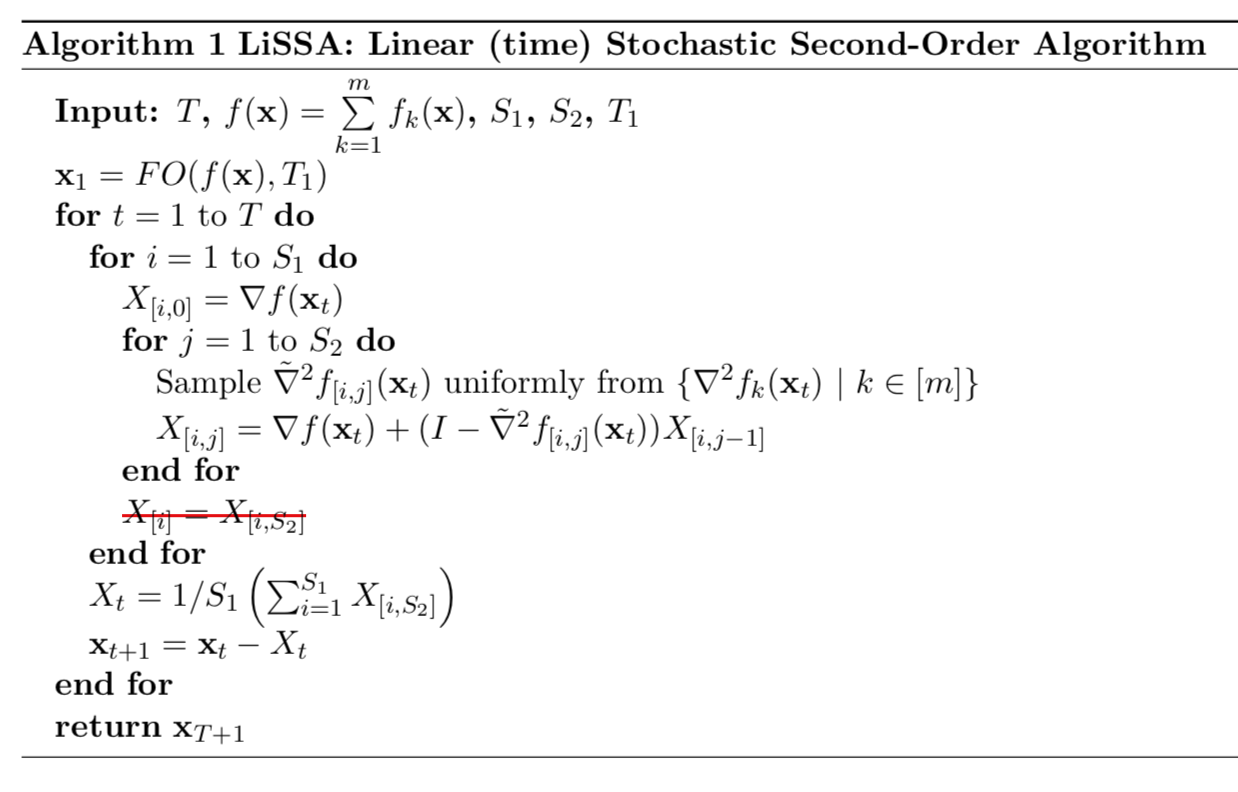
\includegraphics[scale=0.45]{fig/alg1.png}
\end{figure}
\end{frame}


\begin{frame}{2.3. LiSSA —— Theorem}
% 这个定理是分析LiSSA收敛性的,
\examplebox{Theorem 3.3}{
\small
Consider Algorithm 1, and set the parameters as follows:
$$T_{1}=F O\left(M, \hat{\kappa}_{l}\right), S_{1}=O\left(\left(\hat{\kappa}_{l}^{\max }\right)^{2} \ln \left(\frac{d}{\delta}\right)\right), S_{2} \geq 2 \hat{\kappa}_{l} \ln \left(4 \hat{\kappa}_{l}\right).$$

The following guarantee holds for every $t \geq T_{1}$ with probability $1-\delta$
$$\left\|\mathbf{x}_{t+1}-\mathbf{x}^{*}\right\| \leq \frac{\left\|\mathbf{x}_{t}-\mathbf{x}^{*}\right\|}{2}.$$
Moreover, we have that each step of the algorithm takes at most $\tilde{O}\left(m d+\left(\hat{\kappa}_{l}^{\max }\right)^{2} \hat{\kappa}_{l} d^{2}\right)$ time. Additionally, if $f$ is $G L M,$ then each step of the algorithm can be run in time $O\left(m d+\left(\hat{\kappa}_{l}^{\max }\right)^{2} \hat{\kappa}_{l} d\right)$.

}

% 我的参数设定,T1是说我首先要通过一阶算法得到某个精度的解,这个解就是alg中使用的x1,我的T1就是我使用我这个一阶算法,得到x1所用的时间,在这个T1之后,我要用多少时间t-T1来完成我的逼近;(感觉这个一个是证明的精度要求,另一个也和Newton法对初始点的要求有关)

% S1是我给定的,他后来在github上给了代码,默认取得也就只有5,所以其实要求不太高…我试了一下,稍微小一点也可以跑

% s2是为了证bound

% 整个定理的证明有一点复杂;先证明了一个lemma,主要是因为hessian假设了是lipschitz有界的,我得到了一个类似于收敛阶的界限;第二个lemma是想证明,我用来估计的hessian矩阵的逆,与真值的差距的尾部概率,也就是说,这个误差大于某个与S1相关的界限的概率 小于 delta. 这个证明主要用到的是两个

% 进一步给出了Corollary,
\end{frame}
\begin{frame}{2.4. LiSSA —— Corollary}
\examplebox{Corollary 3.4}{For a GLM function $f(\mathbf{x})$ Algorithm 1 returns a point $\mathbf{x}_{t}$ such that with probability at least $1 - \delta$
$$f\left(\mathbf{x}_{t}\right) \leq \min _{\mathbf{x}^{*}} f\left(\mathbf{x}^{*}\right)+\varepsilon$$
in total time $\tilde{O}\left(m+\left(\hat{\kappa}_{l}^{\max }\right)^{2} \hat{\kappa}_{l}\right) d \ln \left(\frac{1}{\varepsilon}\right)$ for $\varepsilon \rightarrow 0$.
}

\end{frame}

\begin{frame}{2.5. LiSSA —— Summary}
\begin{itemize}
	\item Main idea: Tylor Expansion Estimator.
	\item Iteration: in $O(d)$ time.
	\begin{itemize}
		\item Sparsity: in $O(s)$ time.
	\end{itemize}
	\item Convergence: Linear.
	\item Other details:
	\begin{itemize}
		\item Better on condition number, $\kappa_l \leq \kappa$.
		\item Better in high accuracy regime.
		
	\end{itemize}
\end{itemize}
\end{frame}


\begin{frame}{3.1. LiSSA-Sample —— Main Idea}
\begin{itemize}
	\item Much better when $m >> d$.
	\begin{itemize}
		\item Utilize Matrix Sampling Techniques $[CLM+15]$.
	\end{itemize}
\end{itemize}
\begin{figure}
	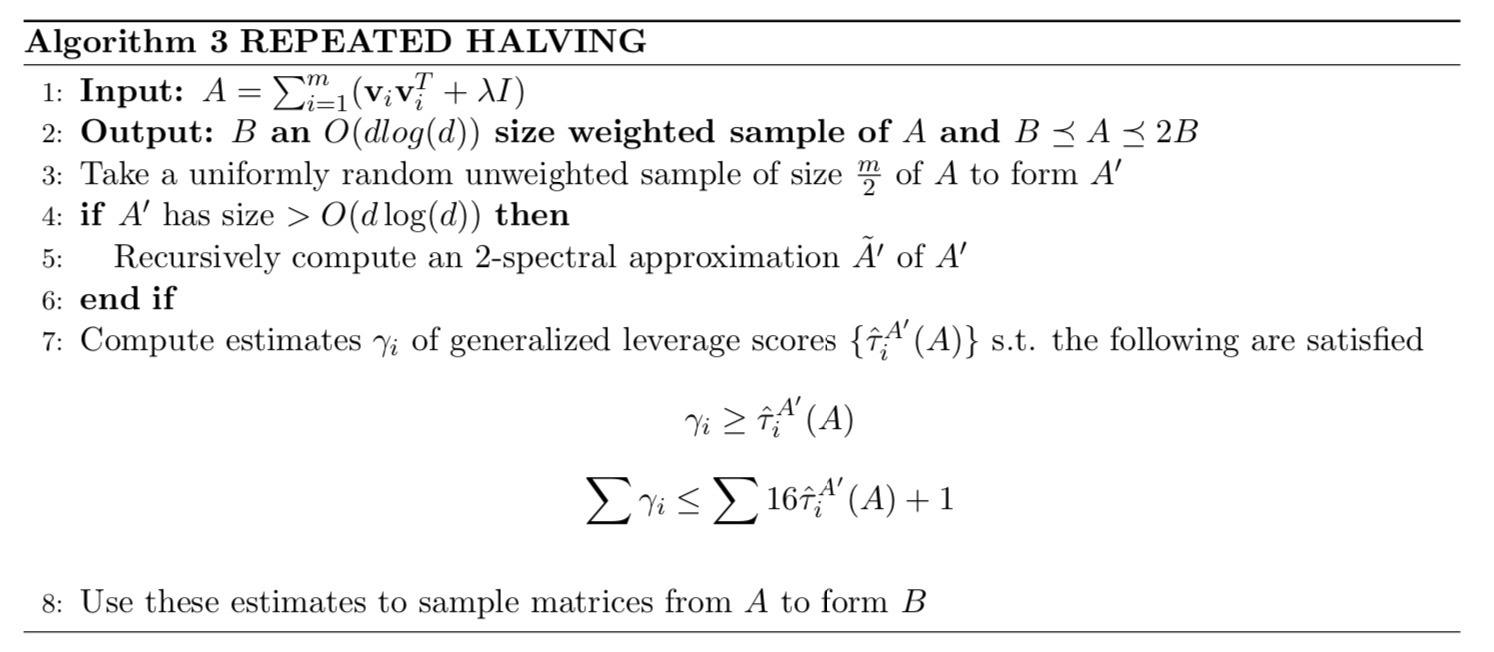
\includegraphics[scale=0.42]{fig/alg3.png}
\end{figure}
\end{frame}


\begin{frame}{3.2. LiSSA-Sample —— Theorem}
\begin{itemize}
	\item \textbf{Time: }$\tilde{O}\left(m d+d \sqrt{\kappa_{\text {sample}}d}\right)$.
	\begin{itemize}
		\item Better condition number, $\kappa_{\text {sample}}$.
	\end{itemize}
\end{itemize}
\begin{figure}
	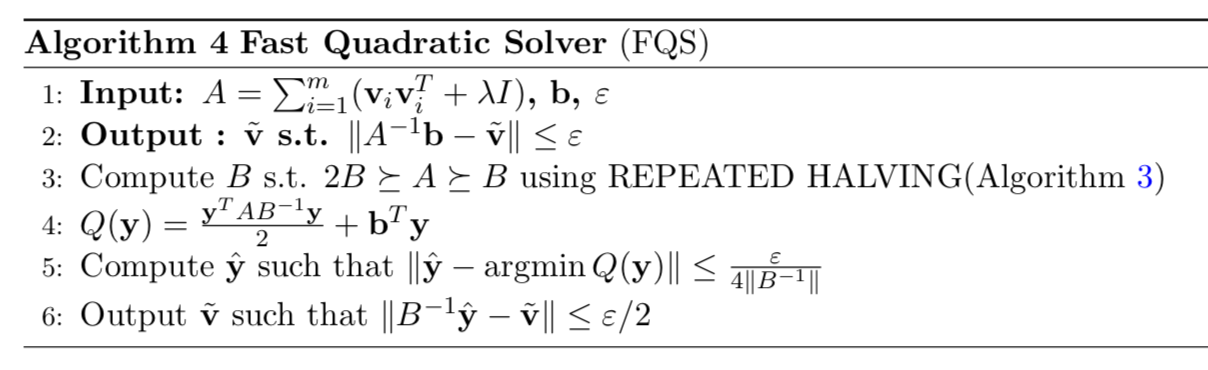
\includegraphics[scale=0.48]{fig/alg4.png}
\end{figure}
\end{frame}


\begin{frame}{4.1. Theoretical Results}

\begin{figure}
	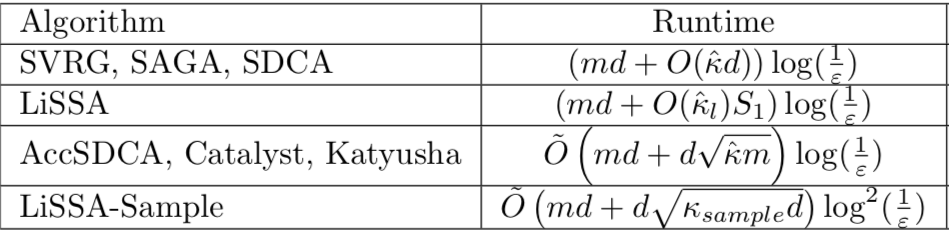
\includegraphics[scale=0.58]{fig/result.png}
\end{figure}
% 理论上讲,lissa是要比一阶算法好的,实验中
% 理论上讲,他的lissa-sample理论上讲,当m>>d的时候,具有最好的时间复杂度
% 要是我的话,我会想让他再比较一下加速的一阶算法和lissasample,他没给

\end{frame}

\begin{frame}{4.2. Empirical Results}

\begin{figure}
	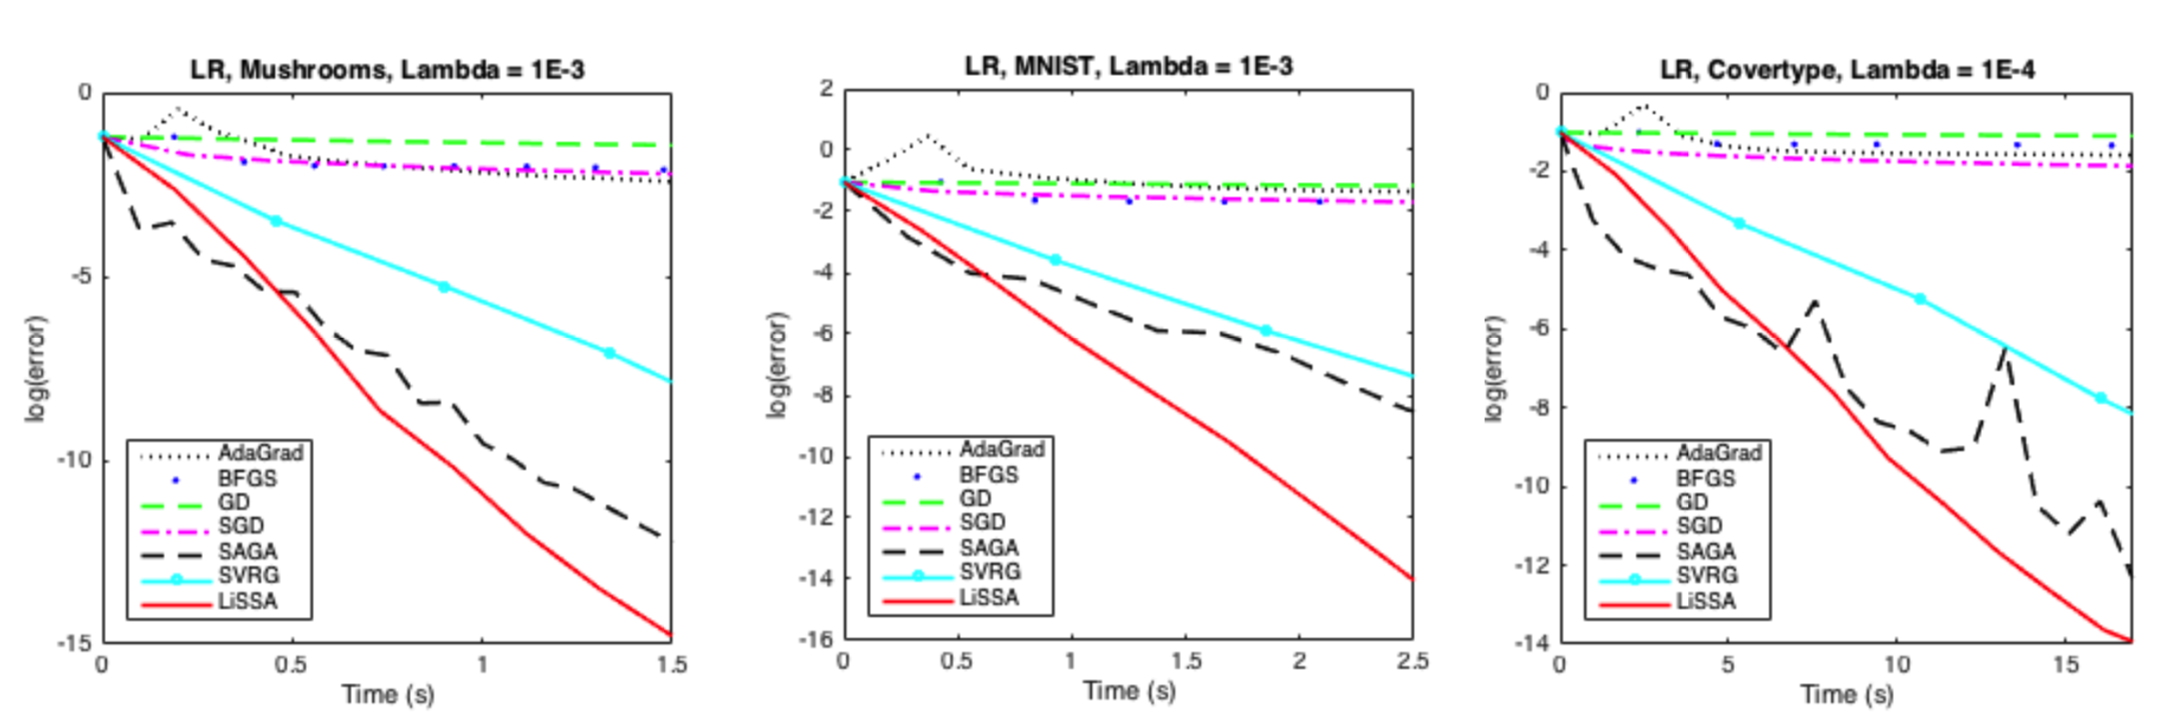
\includegraphics[width = 10cm]{fig/fig2.png}
\end{figure}
\begin{figure}
	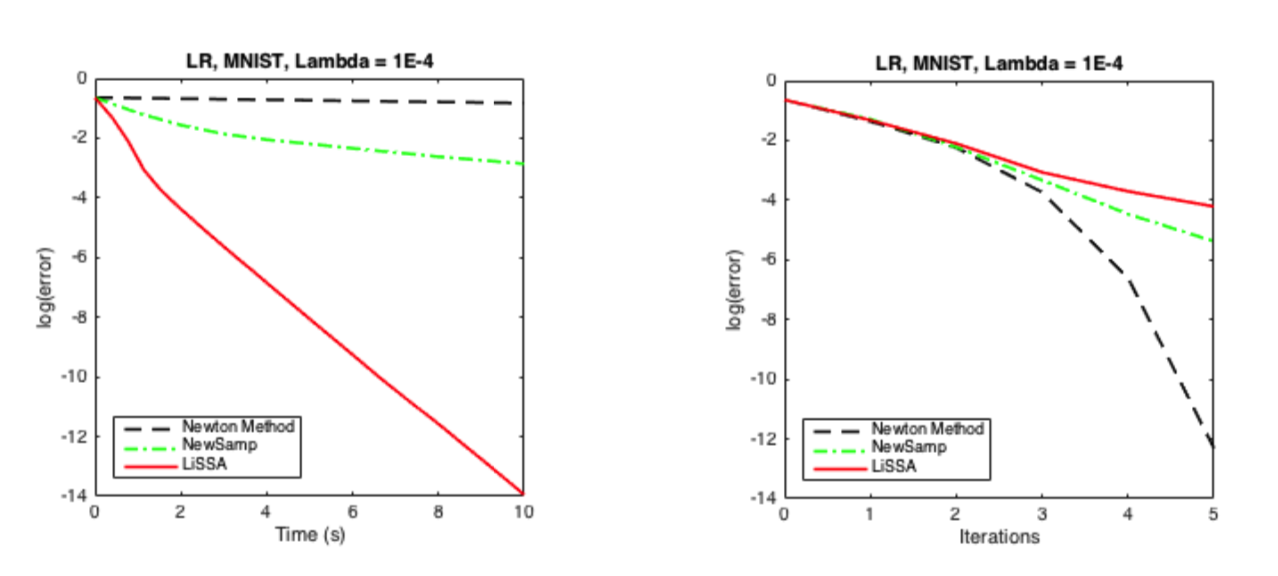
\includegraphics[width = 9cm]{fig/fig3.png}
\end{figure}
\end{frame}


\begin{frame}{}
Thanx  :) !
\end{frame}
\end{document}